\documentclass[10pt]{article}

\usepackage[utf8]{inputenc}
\usepackage[T1]{fontenc}
\usepackage{lmodern}
\usepackage[top=0.55in,bottom=0.5in,left=0.65in,right=0.65in]{geometry}
\usepackage{amsmath,amssymb}
\usepackage{enumitem}
\usepackage{fancyhdr}
\usepackage{titlesec}
\usepackage{tikz}
\usetikzlibrary{arrows.meta,positioning}
\usepackage[hidelinks]{hyperref}

\pagestyle{fancy}
\fancyhf{}
\lhead{\small EECS 3216: Digital Systems Engineering}
\rhead{\small Course Project Proposal}
\renewcommand{\headrulewidth}{0.4pt}
\setlength{\headheight}{13pt}

\setlength{\parindent}{0pt}
\setlength{\parskip}{2pt}
\setlist[itemize]{leftmargin=1.1em,itemsep=0.5pt,topsep=1pt,parsep=0pt}
\titleformat{\section}{\normalsize\bfseries}{\thesection.}{0.4em}{}
\titlespacing*{\section}{0pt}{3pt}{1pt}

% Status tags: every specification item is either already working or proposed.
\newcommand{\built}{\textsf{\scriptsize[built]}}
\newcommand{\prop}{\textsf{\scriptsize[proposed]}}

\newcommand{\proposalheader}[4]{%
\noindent\fbox{\parbox{\dimexpr\textwidth-2\fboxsep-2\fboxrule\relax}{%
\centering{\large\bfseries #1}\\[2pt]
\small\textbf{Target Tier:} #2 \hfill
\textbf{Course:} EECS 3216 (Fall 2026) \hfill
\textbf{Topic:} #3\\[2pt]
\raggedright\footnotesize\textbf{Group Members:} #4
}}\vspace{1pt}}

\begin{document}

\proposalheader
{FPGA Tactical Controller for StarCraft II Micro Scenarios}
{Tier A (100\%)}
{Datapath / Control / VGA}
{Marlin Lachance (213885025), Vaughn Chan (219846914), Hafsa Manazir (219780428), Vladislav Prasko (220741781)}

\section{Overview and Difficulty Justification}
{\small
In the StarCraft II (SC2) mini-game \emph{DefeatRoaches}, friendly Marines fight waves of enemy Roaches.
\built{} A PC sends each game snapshot to the DE10-Lite over UART; the FPGA chooses one attack target per Marine and replies, the PC issues those orders, and VGA draws the units and target lines.
\prop{} A Lanchester strength check and a tactical FSM will also decide \emph{when to disengage}: ATTACK, RETREAT or HOLD.
Tier~A: the UART link, ranking pipeline, FSMs and VGA run concurrently in group-written HDL.

\vspace{2pt}
\begin{center}
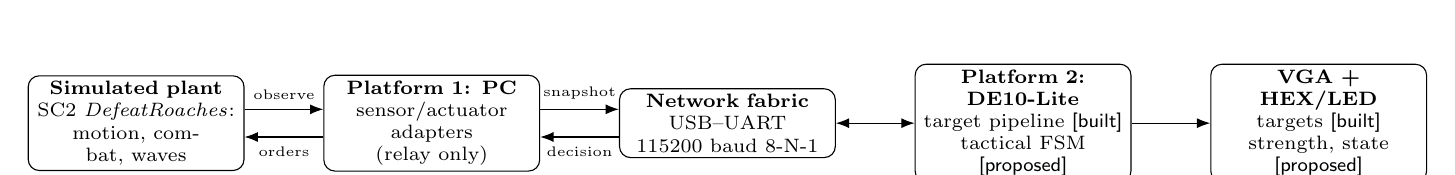
\begin{tikzpicture}[>=Latex,every node/.style={font=\scriptsize,align=center},
box/.style={draw,rounded corners,inner sep=2pt,minimum height=0.75cm}]
\node[box,text width=2.6cm] (plant) {\textbf{Simulated plant}\\SC2 \emph{DefeatRoaches}:\\motion, combat, waves};
\node[box,text width=2.6cm,right=1.0cm of plant] (host) {\textbf{Platform 1: PC}\\sensor/actuator adapters\\(relay only)};
\node[box,text width=2.6cm,right=1.0cm of host] (net) {\textbf{Network fabric}\\USB--UART\\115200 baud 8-N-1};
\node[box,text width=2.6cm,right=1.0cm of net] (fpga) {\textbf{Platform 2: DE10-Lite}\\target pipeline \built\\tactical FSM \prop};
\node[box,text width=2.6cm,right=1.0cm of fpga] (vga) {\textbf{VGA + HEX/LED}\\targets \built\\strength, state \prop};
\draw[->] ([yshift=5pt]plant.east) -- node[above,font=\tiny]{observe} ([yshift=5pt]host.west);
\draw[<-] ([yshift=-5pt]plant.east) -- node[below,font=\tiny]{orders} ([yshift=-5pt]host.west);
\draw[->] ([yshift=5pt]host.east) -- node[above,font=\tiny]{snapshot} ([yshift=5pt]net.west);
\draw[<-] ([yshift=-5pt]host.east) -- node[below,font=\tiny]{decision} ([yshift=-5pt]net.west);
\draw[<->] (net) -- (fpga);
\draw[->] (fpga) -- (vga);
\end{tikzpicture}
\end{center}
\vspace{-5pt}
Adapted from Lee and Seshia, Fig.~1.1~\cite{lee}: SC2 replaces the physical plant, and its observation and order APIs act as sensors and actuators. The PC only relays; every targeting and tactical decision is made on the FPGA.
}

\section{Target Hardware and Peripherals (DE10-Lite Only)}
{\small
\begin{itemize}
\item \textbf{Onboard:} MAX~10 FPGA (\texttt{10M50DAF484C7G}) at 50\,MHz; 2$\times$20 GPIO header (GPIO[0]/[1] = UART RX/TX); VGA port (4-bit RGB); SW4:0; KEY0; HEX5:0; LEDR9:0.
\item \textbf{External:} 3.3\,V USB-to-UART adapter with common ground; 640$\times$480 VGA monitor; PC running SC2 with a Python adapter (\texttt{burnysc2}, \texttt{pyserial}).
\end{itemize}
}

\section{Combinational and Sequential Logic Architecture}
{\small
\begin{itemize}
\item \textbf{Combinational:} \built{} subtractors and multipliers compute the exact squared Marine--Roach distance (no square root); comparators test attack range and compare ranking keys; an 8-bit adder checks each frame's checksum. \prop{} A 17-entry square table and integer comparators evaluate the strength check (Section~4).
\item \textbf{Sequential:} \built{} UART RX/TX FSMs and packet framers; snapshot registers; a three-stage distance/ranking pipeline that accepts one Marine--Roach pair per clock, so one decision takes exactly $n_F n_E + 2$ cycles (at most 258 cycles, 5.16\,\textmu s); VGA timing counters. \prop{} A tactical FSM (ATTACK, RETREAT, HOLD) with a retreat latch, run after target ranking.
\end{itemize}
}

\section{Proposed Extension: Lanchester Strength Check}
{\small
In Lanchester's square law, a side's strength in a ranged fight grows with the square of its unit count; Stanescu et al.\ show such attrition laws predict StarCraft combat~\cite{stanescu}. We use only the square-law strength, not their fitted model:
$P_F = k_F N_F^2$ and $P_E = k_E N_E^2$, where $N \in \{0,\dots,16\}$ counts living units and $k$ is a fixed 16-bit coefficient per side for this matchup (damage rate against opponent health). $N^2$ comes from the table, so products fit in 24 bits with no square root or division.
\textbf{Rule:} latch RETREAT if $4P_F < 3P_E$ (friendly strength below 75\% of enemy) or friendly HP falls to 25\% of its starting total; otherwise ATTACK. HOLD when either side is empty or the retreat reaches its safe point; the latch clears only on reset or a new encounter. A new protocol version adds friendly HP to the request and state, reason and both strengths to the reply.
Cutoffs are our engineering parameters, not from~\cite{stanescu}; the model ignores range, wounds and waves, so retreat is judged by Marines preserved.
}

\section{Concrete Specifications and Testable Features}
{\small
\begin{itemize}
\item \textbf{SC2 targeting and tactical decisions:} \built{} SW0=0: each Marine attacks the nearest Roach. SW0=1, focus fire~\cite{churchill}: the weakest Roach in range, otherwise the nearest. \prop{} ATTACK/RETREAT/HOLD orders from Section~4. \emph{Pass:} board replies match an independent Python reference on every snapshot; retreat preserves more Marines than a no-retreat baseline.
\item \textbf{VGA visualization of controller state:} \built{} 640$\times$480 at 60\,Hz showing units, Marine-to-target lines and policy; HEX5:4 snapshot ID, HEX3 policy, HEX2 status, HEX1:0 the target of the Marine chosen by SW4:1; LEDR shows policy, receive, error and distinct-target count. \prop{} Strength bars, tactical state and reason. \emph{Pass:} for a frozen snapshot, the display matches the reply frame.
\item \textbf{UART communication:} \built{} 115200 baud 8-N-1, one request and one reply, up to 16 units per side (151-byte request, 13.1\,ms). Checksum, count, range and 10\,ms timeout checks; a bad frame gets an error status and never changes the display. \emph{Pass:} a corrupted frame is rejected and the next valid frame is processed without reset; every reply reports datapath cycles.
\item \textbf{Originality:} all HDL (UART, framers, pipeline, FSMs, VGA) is group-written; the PC adapter uses \texttt{burnysc2}/\texttt{pyserial} and Blizzard's map.
\end{itemize}
}

\section{Verification Plan and Team Task Allocation}
{\small
\textbf{Marlin Lachance (lead):} existing pipeline, architecture, tactical FSM, SC2 host integration.
\textbf{Vaughn Chan (hardware):} board setup, UART/VGA verification, strength and state displays.
\textbf{Hafsa Manazir (documentation):} report, references, results.
\textbf{Vladislav Prasko (demonstration):} SC2 scenarios, integration testing, evidence, presentation.
We also report Quartus timing/resources, datapath cycles and UART latency, and claim no CPU speedup (the 13.1\,ms link dominates).
}

\vspace{-3pt}
{\scriptsize
\renewcommand{\section}[2]{}% no "References" heading: keep the proposal to one page
\begin{thebibliography}{3}
\setlength{\itemsep}{-2pt}
\bibitem{lee} E. A. Lee and S. A. Seshia, \textit{Introduction to Embedded Systems: A Cyber-Physical Systems Approach}, 2nd ed., MIT Press, 2017, Fig.~1.1.
\bibitem{churchill} D. Churchill and M. Buro, ``Portfolio Greedy Search and Simulation for Large-Scale Combat in StarCraft,'' \textit{IEEE CIG}, 2013, Sec.~III.
\bibitem{stanescu} M. Stanescu, N. Barriga and M. Buro, ``Using Lanchester Attrition Laws for Combat Prediction in StarCraft,'' \textit{AIIDE}, 2015.
\end{thebibliography}
}

\end{document}
